%!TEX program = xelatex
\documentclass[12pt,oneside]{ctexbook}

% ---------- 基础宏包 ----------
\usepackage{amsmath, amssymb, amsthm}
\usepackage{graphicx}
\usepackage{hyperref}
\usepackage{geometry}
\usepackage{fancyhdr}
\usepackage{setspace}

% 页面设置
\geometry{a4paper, margin=2.5cm}
\setstretch{1.3}

% 页眉页脚
\pagestyle{fancy}
\fancyhf{}
\fancyhead[L]{深度学习与计算物理(翻译)}
\fancyhead[R]{\leftmark}
\fancyfoot[C]{\thepage}

% 超链接美化
\hypersetup{
    colorlinks=true,
    linkcolor=blue,
    citecolor=blue,
    urlcolor=blue
}

% ---------- 自定义环境 ----------
\newenvironment{mycomment}{
    \begin{quote}
    \textbf{我的理解与注释:}\par
}{\end{quote}}

% ---------- 封面 ----------
\title{深度学习与计算物理 \\[8pt]
\Large 翻译与学习笔记}
\author{Linus}
\date{\today}

\begin{document}
\maketitle
\tableofcontents
\newpage

% ---------- 引入章节 ----------
\chapter{引言}
\label{chap:introduction}

统计学习和数据驱动算法的理论与方法可以追溯到19世纪初。但现代机器学习的最初萌芽可以追溯到1943年McCulloch和Pitts的研究工作\cite{mcculloch1943},他们提出了第一个\term{人工神经元}{Artificial Neuron}模型,该模型松散地基于脊椎动物生物神经元的功能。Arthur Samuel被普遍认为是在1959年首次提出"机器学习"这一术语的人,当时他在IBM从事教计算机下跳棋的研究工作\cite{samuel1959}。机器学习在计算机视觉、语音识别和自然语言处理等应用领域取得了巨大成功。但近年来也见证了\term{机器学习}{Machine Learning}(特别是深度学习)算法在解决物理驱动问题方面的兴起,如逼近偏微分方程的解和反问题。

本课程涉及的主题位于\term{计算物理}{Computational Physics}和机器学习的交叉领域。在我们能够理解结合这两个重要概念的必要性之前,我们需要分别理解它们各自的含义。

\section{计算物理}
\label{sec:computational_physics}

计算物理在解决科学和工程领域的许多问题中发挥着基础性作用。为了理解这一概念,我们简要概述解决物理问题所涉及的关键步骤:

\begin{enumerate}
\item 考虑某个物理现象,并收集感兴趣的可观测量的测量数据。例如,在研究海洋波浪时,从海洋浮标获得的水位高度和波浪方向的测量数据。

\item 基于观测结果,假设一个物理定律。例如,你观察到在封闭系统中流体的总质量在任何时候都是守恒的。

\item 写下该定律的数学描述。这可能使用\term{常微分方程}{Ordinary Differential Equations, ODEs}、\term{偏微分方程}{Partial Differential Equations, PDEs}、积分方程等。

\item 一旦数学模型建立,求解系统的解。有两种方法可以获得解:
    \begin{enumerate}[label=(\alph*)]
    \item 在某些情况下,可以得到解的精确解析形式。例如,可以使用分离变量法、拉普拉斯变换、傅里叶变换或积分因子来求解常微分方程/偏微分方程。
    
    \item 在大多数情况下,无法得到解的精确表达式,必须使用数值算法进行适当的近似。例如,可以使用前向或后向欧拉法、中点法则或\term{龙格-库塔格式}{Runge-Kutta Schemes}来求解常微分方程组\cite{burden2015};或者可以使用\term{有限差分/体积/元素方法}{Finite Difference/Volume/Element Methods}来求解偏微分方程\cite{strikwerda2004}。
    \end{enumerate}

\item 一旦设计出评估解(精确或近似)的算法,就使用它来验证数学模型,即查看预测是否与收集的数据一致。
\end{enumerate}

所有这些步骤广泛地描述了计算物理学所包含的内容。

\section{机器学习}
\label{sec:machine_learning}

与计算物理不同,\term{机器学习}{Machine Learning, ML}不需要假设物理定律。涉及的一般步骤是:

\begin{enumerate}
\item 通过观察物理现象、通过某些可观测量的实时测量或使用数值求解器逼近现象来收集数据。

\item 使用收集的数据训练合适的算法,目的是发现各个样本之间的模式或关系。具体例子见第\ref{subsec:ml_examples}节。

\item 一旦训练完成,使用机器学习算法进行未来预测,并用额外收集的数据进行验证。
\end{enumerate}

\subsection{机器学习的例子}
\label{subsec:ml_examples}

\begin{enumerate}
\item \textbf{回归算法:}给定成对数据集$\{(x_i, y_i) : 1 \leq i \leq N\}$,它对应于某个未知函数$y = f(x)$,对该数据集拟合多项式(或任何其他基函数)以便逼近$f$。例如,找到线性拟合的系数$a, b$:
\begin{equation}
\tilde{f}(x; a, b) = ax + b
\end{equation}
以最小化误差
\begin{equation}
\Pi(a, b) = \sum_{i=1}^{N} |y_i - \tilde{f}(x_i)|^2
\label{eq:regression_error}
\end{equation}

如果$(a^*, b^*) = \arg\min_{a,b} \Pi(a, b)$,那么我们可以认为$\tilde{f}^*(x) := \tilde{f}(x; a^*, b^*)$是$f(x)$的近似(见图\ref{fig:ml_examples}a)。

\item \textbf{决策树:}给定来自样本人群的数据集,包含特征:年龄和收入。此外,数据被分为两组;A组中的个体拥有房屋,而B组中的个体没有。然后,给定新数据点的特征,我们希望预测这个新个体拥有房屋的概率。决策树可以用来解决这个分类问题。典型决策树的工作方式是通过做出能够最大化数据集中样本的基于组的分离的切分(见图\ref{fig:ml_examples}b)。然后,基于这些切分,算法确定新点属于特定类别/组的概率。

\item \textbf{聚类算法:}给定具有每个样本多个特征的数据集,在数据中寻找簇/模式(见图\ref{fig:ml_examples}c)。
\end{enumerate}

\begin{figure}[H]
\centering
% \includegraphics[width=\textwidth]{figures/ml_examples.png}
\begin{tikzpicture}[scale=0.8]
% 这里应该包含图1.1的绘制代码,展示三个子图:
% (a) 回归示例 (b) 决策树示例 (c) 聚类示例
% 由于原图较复杂,这里用占位符表示
\draw (0,0) rectangle (12,4);
\node at (2,2) {(a) 回归};
\node at (6,2) {(b) 决策树};
\node at (10,2) {(c) 聚类};
\end{tikzpicture}
\caption{机器学习的例子}
\label{fig:ml_examples}
\end{figure}

\subsection{基于任务的机器学习算法类型}
\label{subsec:ml_types}

广义上讲,有四种类型的机器学习算法:

\begin{enumerate}
\item \textbf{监督学习:}给定数据$S = \{(x_i, y_i) : 1 \leq i \leq N\}$,对某个新的$\hat{x}$预测$\hat{y}$,使得$(\hat{x}, \hat{y}) \notin S$。例如,给定一组图像和图像标签(如狗、猫、牛等),训练分类机器学习算法学习图像和标签之间的关系,并使用它来预测新图像的标签。

\item \textbf{无监督学习:}给定数据$S = \{x_i \in \Omega_x : 1 \leq i \leq N\}$,在$\Omega_x$的不同区域之间寻找关系。例如,在数据集中寻找簇,或找到控制该数据分布的概率分布$p_x(x)$的表达式并从中生成新样本。

\item \textbf{半监督学习:}这类方法介于监督学习和无监督学习之间。它们通常使用标记和未标记数据的组合进行训练。例如,我们有10,000张未标记的图像和只有50张标记的图像。我们能使用这个数据集开发图像分类算法吗?

\item \textbf{强化学习:}属于这一类的方法基于对所做决策的奖励或惩罚进行学习。因此,学习适当的路径/策略以最大化奖励。这种策略可用于训练算法下象棋或围棋。
\end{enumerate}

在本课程中,我们将主要关注前两种类型的机器学习算法。

\section{人工智能、机器学习和深度学习}
\label{sec:ai_ml_dl}

有时,\term{人工智能}{Artificial Intelligence, AI}、机器学习和\term{深度学习}{Deep Learning, DL}这些术语被互换使用。实际上,这些是三个相关但不同的概念。这可以通过查看图\ref{fig:ai_ml_dl_venn}中的韦恩图来理解。

\begin{figure}[H]
\centering
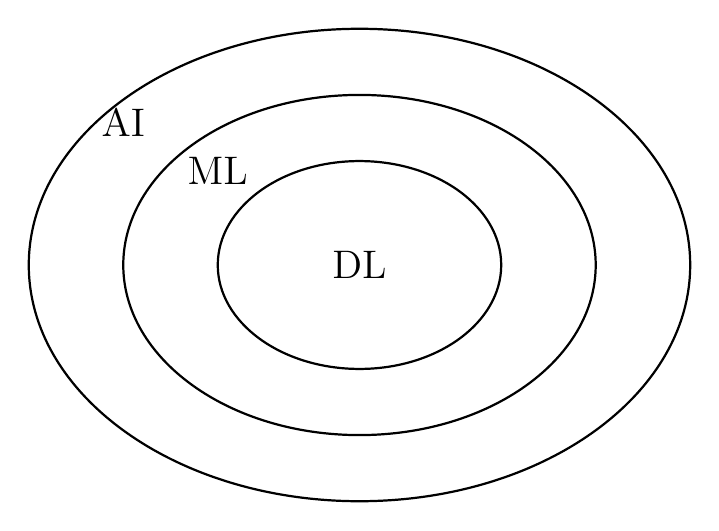
\begin{tikzpicture}[scale=1.2]
% 绘制三个相互嵌套的椭圆
\draw[thick] (0,0) ellipse (3.5cm and 2.5cm);
\draw[thick] (0,0) ellipse (2.5cm and 1.8cm);
\draw[thick] (0,0) ellipse (1.5cm and 1.1cm);

% 添加标签
\node at (-2.5,1.5) {\Large AI};
\node at (-1.5,1) {\Large ML};
\node at (0,0) {\Large DL};
\end{tikzpicture}
\caption{AI、ML和DL之间的关系}
\label{fig:ai_ml_dl_venn}
\end{figure}

AI指的是具有类人智能的系统。虽然机器学习是AI系统的关键组成部分,但还涉及其他要素。自动驾驶汽车是AI的原型例子。让我们仔细看看这样一个系统的设计(见图\ref{fig:self_driving_car})。汽车配备了摄像头,可以拍摄前方道路的实时图像/视频。然后将这些帧传递给执行\term{语义分割}{Semantic Segmentation}的机器学习算法,即分割出帧的不同区域并对每个区域中的对象类型(汽车、树、道路、天空等)进行分类。一旦完成这种分割,就将其传递给决策系统,该系统基于这个分割图像决定汽车的下一个动作应该是什么。然后这个信息通过控制模块,实际控制汽车的机械动作。整个过程模拟了真实驾驶员的行为,因此是人工智能。

\begin{figure}[H]
\centering
\begin{tikzpicture}[node distance=2cm, auto]
% 定义节点样式
\tikzstyle{block} = [rectangle, draw, fill=blue!20, text width=2cm, text centered, minimum height=1cm]
\tikzstyle{line} = [draw, -latex']

% 绘制流程图
\node [block] (camera) {摄像头};
\node [block, right of=camera] (segmenter) {语义分割器};
\node [block, right of=segmenter] (decision) {决策系统};
\node [block, right of=decision] (control) {控制模块};

% 连接节点
\path [line] (camera) -- (segmenter);
\path [line] (segmenter) -- (decision);
\path [line] (decision) -- (control);

% 添加标签
\node [below of=camera, node distance=1cm] {实时图像};
\node [below of=segmenter, node distance=1cm] {分割图像};
\node [below of=decision, node distance=1cm] {动作决策};
\node [below of=control, node distance=1cm] {机械控制};
\end{tikzpicture}
\caption{自动驾驶汽车AI系统示意图}
\label{fig:self_driving_car}
\end{figure}

另一方面,机器学习(ML)是该系统中使用数据训练的组件。也就是说,它们通过数据学习。在上面的例子中,语义分割器就是这样一个系统。有许多机器学习算法可以使用数据执行这项任务,我们将在本课程中学习其中的一些。决策系统也可能是ML组件——在这里,要做出的适当决策是从先前的数据中学到的。然而,它也可能是基于规则的非ML专家系统。

深度学习是机器学习算法的一个子集。最简单形式的深度学习架构,称为\term{前馈网络}{Feed-forward Network},包含多个非线性变换层。这种架构松散地受到信号如何在生物体的中枢神经系统中传输的启发。我们将在第2章更详细地研究深度学习架构。

\section{机器学习与计算物理}
\label{sec:ml_cp_combination}

现在我们对计算物理和机器学习有了更好的理解,下一个显而易见的问题是"我们为什么需要看两者的结合?"我们在下面列出几个动机:

\begin{itemize}
\item 对于"物理"数据的复杂模式,机器学习提供了表示数学定律的替代途径。考虑包含两个重要组件的物理过程。其中,一个得到很好理解并具有可信的数学模型,另一个理解不充分且没有数学描述。在这种情况下,可以对第一个组件使用计算物理,对第二个组件使用机器学习。这方面的具体例子是受能量守恒和复杂本构模型支配的系统。对于前者,我们可能有一个很好理解的数学模型,而对于后者,我们可能必须依赖机器学习来开发模型。

\item 机器学习通常非常依赖数据。但物理知识可以帮助限制输入和解/预测所在的\term{流形}{Manifold}。有了这样的约束,我们可以减少训练机器学习算法所需的数据量。

\item 用于分析计算物理的工具(\term{泛函分析}{Functional Analysis}、数值分析、精确解收敛的概念、概率框架)可以转移到机器学习中。将这些工具应用于机器学习有助于我们更好地理解和设计更好的机器学习算法。
\end{itemize}

我们简要总结本课程将涵盖的各种主题:

\begin{itemize}
\item \term{深度神经网络}{Deep Neural Networks}(多层感知器)及其收敛性。
\item \term{随机梯度下降}{Stochastic Gradient Descent}及其与常微分方程的关系。
\item \term{残差网络}{Residual Networks, ResNets}及其与非线性常微分方程的联系(\term{神经常微分方程}{Neural ODEs})。
\item \term{卷积神经网络}{Convolutional Neural Networks}及其与偏微分方程的联系。
\item 用于求解偏微分方程的深度学习算法。
\item 用于逼近算子的深度学习算法。
\item \term{生成算法}{Generative Algorithms}及其与计算物理的联系。
\item 用于求解概率反问题的生成算法。
\end{itemize}

\section{计算练习}
\label{sec:computational_exercises}

为了有效使用本课程中讨论的各种机器学习算法并解决计算练习,需要很好地掌握Python编程和PyTorch。下面列出了关于必要编程概念的各种资源和教程。

\begin{enumerate}
\item \textbf{Python基础、NumPy和绘图:}对于那些从未使用过Python的人,或者甚至对于那些熟悉Python并想要更新编程知识的人来说,一个很好的资源是\url{https://www.w3schools.com/python/}。本教程涵盖了重要的Python模块,如NumPy、Pandas和SciPy,描述了如何使用Matplotlib生成图表,以及如何读/写文件。

\item \textbf{PyTorch:}本课程中使用的代码将使用PyTorch编写,这是一个最初由Meta AI开发的机器学习框架。您可以按照这里给出的说明在您的机器上本地安装PyTorch:\url{https://pytorch.org/get-started/locally/}。关于使用PyTorch的各种教程可以在这里找到:\url{https://pytorch.org/tutorials/}。

\item \textbf{Google Colab:}如果您不希望在本地安装PyTorch,或者没有适当的硬件来训练深度学习模型,您也可以使用Google Colab:\url{https://colab.research.google.com}。Colab本质上是Jupyter notebook和Google Drive的组合,只需要您有一个Google账户。Colab吸引人的地方在于它预装了许多有用的包(如NumPy、PyTorch等),所以每个人都可以使用它而无需担心安装正确版本的库和依赖项。此外,它完全在云端运行,可以直接通过Web浏览器启动和使用。它还提供对强大GPU和TPU的免费访问。
\end{enumerate}

\subsection{环境设置建议}
\label{subsec:environment_setup}

对于初学者,我们建议按照以下顺序学习:

\begin{enumerate}
\item 首先熟悉Python基础语法和NumPy数组操作
\item 学习Matplotlib进行数据可视化
\item 了解PyTorch张量的基本操作
\item 学习如何构建和训练简单的神经网络
\item 实践本书中的编程练习
\end{enumerate}

\section{小结}
\label{sec:summary}

本章介绍了深度学习和计算物理领域的基础概念。我们探讨了:

\begin{itemize}
\item 计算物理的基本方法论及其在科学问题求解中的作用
\item 机器学习的不同类型及其应用领域
\item 人工智能、机器学习和深度学习之间的层次关系
\item 将机器学习与计算物理相结合的动机和潜在优势
\item 本课程将涵盖的主要主题概览
\end{itemize}

在接下来的章节中,我们将深入探讨深度神经网络的数学基础,学习各种训练技术,并将这些方法应用于具体的物理问题。我们将看到机器学习如何为传统的计算物理方法提供新的视角,以及物理直觉如何帮助我们设计更好的机器学习算法。

\newpage
\chapter{深度神经网络简介}

\section{多层感知机(MLP)结构}
MLP 的目标是近似函数 $f: \mathbb{R}^d \to \mathbb{R}^D$。其基本单元是人工神经元,由若干层堆叠组成。

\begin{mycomment}
在这一部分,我发现 MLP 的结构与“线性代数中的仿射变换 + 非线性函数”非常类似。  
可以把它理解为“线性映射 + 激活函数”的交替堆叠。  
\end{mycomment}

\newpage

\chapter{残差神经网络}
\label{chap:residual_networks}

\term{残差网络}{Residual Networks}(或ResNets)由He等人在2015年提出。在本章中,我们将讨论这些网络是什么,为什么引入它们以及它们与常微分方程的关系。

\section{深度网络中的梯度消失}
\label{sec:vanishing_gradients}

在训练神经网络时,梯度$\frac{\partial\Pi}{\partial W^{(l)}}$、$\frac{\partial\Pi}{\partial b^{(l)}}$可能变得非常小。例如,考虑一个非常深的网络,假设$L \geq 20$。如果对于$l \leq \bar{l}$有$\left|\left|\frac{\partial\Pi}{\partial W^{(l)}}\right|\right| << 1$,那么网络前$\bar{l}$层的贡献将是微不足道的,因为它们的权重对损失函数的影响很小。由于这种深度截断,深度网络在表达能力方面的优势就丧失了。

那么为什么会发生这种情况呢?回想第2.8节中的
\begin{equation}
\frac{\partial\Pi}{\partial W^{(l)}} = \frac{\partial\Pi}{\partial\xi^{(l)}} \otimes x^{(l-1)}
\end{equation}
以及
\begin{equation}
\frac{\partial\Pi}{\partial\xi^{(l)}} = S^{(l)} \prod_{m=l+1}^{L+1} \left(W^{(m)T} S^{(m)}\right) \frac{\partial\Pi}{\partial x^{(L+1)}}
\label{eq:gradient_chain}
\end{equation}

对于任何矩阵$A$,设$\tau(A)$表示最大奇异值。那么我们可以界定$\left|\left|\frac{\partial\Pi}{\partial\xi^{(l)}}\right|\right|$为
\begin{equation}
\left|\left|\frac{\partial\Pi}{\partial\xi^{(l)}}\right|\right| \leq \tau(S^{(l)}) \prod_{m=l+1}^{L+1} \left(\tau(W^{(m)}) \tau(S^{(m)})\right) \left|\left|\frac{\partial\Pi}{\partial x^{(L+1)}}\right|\right|
\label{eq:gradient_bound}
\end{equation}

回想$S^{(m)} \equiv \text{diag}[\sigma'(\xi_1^{(m)}), \ldots, \sigma'(\xi_{H_l}^{(m)})]$,其中$\sigma'$表示$\sigma$对其参数的导数。对于ReLU,其值要么是0要么是1。因此$\tau(S^{(m)}) = 1$。

另外,为了稳定性,我们希望$\tau(W^{(m)}) < 1$。否则网络的输出可能变得无界。在实践中,这可以通过在损失函数中增加正则化项来强制实现。因此,方程(\ref{eq:gradient_bound})简化为
\begin{equation}
\left|\left|\frac{\partial\Pi}{\partial\xi^{(l)}}\right|\right| \leq \prod_{m=l+1}^{L+1} \left(\tau(W^{(m)})\right) \left|\left|\frac{\partial\Pi}{\partial x^{(L+1)}}\right|\right|
\label{eq:gradient_bound_simplified}
\end{equation}

其中乘积中的每一项都是小于1的标量。随着项数的增加,即$L - l >> 1$,这个乘积可能,而且确实会变得非常小。这通常发生在$L - l \approx 20$时,在这种情况下$\left|\left|\frac{\partial\Pi}{\partial\xi^{(l)}}\right|\right|$,因此$\left|\left|\frac{\partial\Pi}{\partial W^{(l)}}\right|\right|$变得非常小。这个问题被称为\term{梯度消失问题}{Vanishing Gradients Problem}。它在深度网络中表现为内部层(比如$L - l > 20$)的权重对网络没有贡献。

在\cite{he2015}中,作者证明了采用更深的网络实际上可能导致训练和验证误差的增加。为了证明这一点,我们训练不同深度的多层感知器来逼近函数
\begin{equation}
u(x) = \sin\left(\frac{2\pi(x + 1)}{3}\right) \cos(2\pi x), \quad x \in [0, 1]
\label{eq:target_function}
\end{equation}

如图\ref{fig:mlp_performance_train}和图\ref{fig:mlp_performance_test}的第一列所示,随着多层感知器深度的增加,训练和测试(均方误差)损失曲线向上移动。就预测而言,只有深度=10才能很好地逼近函数。深度=20时,对域右侧(高频模式占主导)的逼近很差。如果我们将深度增加到40,多层感知器似乎学习了一个常数函数。因此,超过某个点,增加网络的深度可能适得其反。基于我们之前关于梯度消失的讨论,我们知道为什么会这样。鉴于此,我们希望提出一种网络架构,通过确保$\left|\left|\frac{\partial\Pi}{\partial x^{(L+1)}}\right|\right| \approx \left|\left|\frac{\partial\Pi}{\partial\xi^{(1)}}\right|\right|$来解决梯度消失问题。

这意味着要求当网络权重趋近于小值时,网络应该趋近于恒等映射,而不是零映射。这就是ResNet架构背后的核心思想。

\begin{figure}[H]
\centering
\begin{tikzpicture}[scale=0.8]
% 左侧:无残差连接
\begin{scope}
\draw (0,0) rectangle (6,4);
\node at (3,2) {\parbox{5cm}{\centering 无残差连接的MLP性能\\(训练集)}};
\node at (3,0.5) {深度增加 $\rightarrow$ 性能下降};
\end{scope}

% 右侧:有残差连接
\begin{scope}[xshift=7cm]
\draw (0,0) rectangle (6,4);
\node at (3,2) {\parbox{5cm}{\centering 有残差连接的MLP性能\\(训练集)}};
\node at (3,0.5) {深度增加 $\rightarrow$ 性能稳定};
\end{scope}
\end{tikzpicture}
\caption{在训练集上,无残差连接(左)和有残差连接(右)的MLP在逼近式(\ref{eq:target_function})时随深度增加的性能表现}
\label{fig:mlp_performance_train}
\end{figure}

\begin{figure}[H]
\centering
\begin{tikzpicture}[scale=0.8]
% 左侧:无残差连接
\begin{scope}
\draw (0,0) rectangle (6,4);
\node at (3,2) {\parbox{5cm}{\centering 无残差连接的MLP性能\\(测试集)}};
\node at (3,0.5) {深度增加 $\rightarrow$ 泛化能力差};
\end{scope}

% 右侧:有残差连接
\begin{scope}[xshift=7cm]
\draw (0,0) rectangle (6,4);
\node at (3,2) {\parbox{5cm}{\centering 有残差连接的MLP性能\\(测试集)}};
\node at (3,0.5) {深度增加 $\rightarrow$ 泛化能力好};
\end{scope}
\end{tikzpicture}
\caption{在测试集上,无残差连接(左)和有残差连接(右)的MLP在逼近式(\ref{eq:target_function})时随深度增加的性能表现}
\label{fig:mlp_performance_test}
\end{figure}

\section{残差网络}
\label{sec:resnets}

考虑一个深度为6的多层感知器(如图\ref{fig:resnet_structure}所示),每个隐藏层都有固定的宽度$H$。我们以以下方式在隐藏层之间添加\term{跳跃连接}{Skip Connections}:
\begin{equation}
x_i^{(l)} = \sigma(W_{ij}^{(l)} x_j^{(l-1)} + b_i^{(l)}) + x_i^{(l-1)}, \quad 2 \leq l \leq L
\label{eq:resnet_equation}
\end{equation}

我们可以做出以下观察:

\begin{enumerate}
\item 如果所有权重(和偏置)都为零,那么$x^{(5)} = x^{(1)}$,这反过来意味着
\begin{equation}
\frac{\partial\Pi}{\partial x^{(1)}} = \frac{\partial\Pi}{\partial x^{(5)}}
\end{equation}
即,我们不会有梯度消失的问题。

\item ResNet前向和反向传播的\term{计算图}{Computational Graph}如图\ref{fig:resnet_computational_graph}所示。观察这个图,很明显现在$\frac{\partial x^{(l+1)}}{\partial x^{(l)}}$的表达式涉及遍历两个分支并将它们的和相加。因此,我们有
\begin{equation}
\frac{\partial\Pi}{\partial\xi^{(l)}} = S^{(l)} \prod_{m=l+1}^{L+1} \left(I + W^{(m)T} S^{(m)}\right) \frac{\partial\Pi}{\partial x^{(L+1)}}
\label{eq:resnet_gradient}
\end{equation}

现在,如果我们通过正则化假设$\|W^{(m)}\| << 1$,我们有
\begin{equation}
\frac{\partial\Pi}{\partial\xi^{(l)}} = S^{(l)} \left(I + \sum_{m=l+1}^{L+1} W^{(m)T} S^{(m)} + \text{高阶项}\right) \frac{\partial\Pi}{\partial x^{(L+1)}}
\label{eq:resnet_gradient_approximation}
\end{equation}

在上面的表达式中,即使各个矩阵的元素很小,它们的和不一定趋近于零矩阵。这意味着我们可以在输入层和输出层附近的梯度之间创建有限(且显著)的变化,同时仍然要求权重很小(通过正则化)。
\end{enumerate}

\begin{figure}[H]
\centering
\begin{tikzpicture}[node distance=1.5cm, auto]
% 定义节点样式
\tikzstyle{layer} = [circle, draw, fill=blue!20, minimum size=0.8cm]
\tikzstyle{input} = [circle, draw, fill=green!20, minimum size=0.8cm]
\tikzstyle{output} = [circle, draw, fill=red!20, minimum size=0.8cm]
\tikzstyle{line} = [draw, -latex']
\tikzstyle{skip} = [draw, -latex', dashed, red]

% 输入层
\node [input] (x0) {$x^{(0)}$};

% 隐藏层
\node [layer, right of=x0] (x1) {$x^{(1)}$};
\node [layer, right of=x1] (x2) {$x^{(2)}$};
\node [layer, right of=x2] (x3) {$x^{(3)}$};
\node [layer, right of=x3] (x4) {$x^{(4)}$};
\node [layer, right of=x4] (x5) {$x^{(5)}$};

% 输出层
\node [output, right of=x5] (x6) {$x^{(6)}$};

% 正常连接
\path [line] (x0) -- (x1);
\path [line] (x1) -- (x2);
\path [line] (x2) -- (x3);
\path [line] (x3) -- (x4);
\path [line] (x4) -- (x5);
\path [line] (x5) -- (x6);

% 跳跃连接(修正:使用 bend right 而不是 bend above)
\path [skip] (x0) to[bend right] (x2);
\path [skip] (x1) to[bend right] (x3);
\path [skip] (x2) to[bend right] (x4);
\path [skip] (x3) to[bend right] (x5);
\path [skip] (x4) to[bend right] (x6);

% 标签
\node [below of=x3, node distance=2cm] {深度为6的残差网络,带有跳跃连接};
\end{tikzpicture}
\caption{深度为6的残差网络,带有跳跃连接}
\label{fig:resnet_structure}
\end{figure}

\begin{figure}[H]
\centering
\begin{tikzpicture}[node distance=2cm, auto]
% 定义节点样式
\tikzstyle{block} = [rectangle, draw, fill=blue!20, text width=2.5cm, text centered, minimum height=1cm]
\tikzstyle{sum} = [circle, draw, fill=yellow!20, minimum size=0.8cm]
\tikzstyle{line} = [draw, -latex']
\tikzstyle{skip} = [draw, -latex', red]

% 前向传播路径
\node [block] (f1) {$\sigma(W^{(l)}x + b^{(l)})$};
\node [sum, right of=f1] (sum1) {$+$};

% 连接
\path [line] (f1) -- (sum1);

% 输入输出
\node [left of=f1, node distance=3cm] (input) {$x^{(l-1)}$};
\node [right of=sum1, node distance=2cm] (output) {$x^{(l)}$};

\path [line] (input) -- (f1);
\path [line] (sum1) -- (output);
\path [skip] (input) -- (sum1) node[midway, above] {恒等映射};

% 标签
\node [below of=f1, node distance=2cm] {残差网络前向和反向传播的计算图};
\end{tikzpicture}
\caption{残差网络前向和反向传播的计算图}
\label{fig:resnet_computational_graph}
\end{figure}

我们通过训练不同深度的多层感知器来逼近式(\ref{eq:target_function})来经验性地证明添加残差跳跃连接的好处,但现在在隐藏层之间包括跳跃连接。图\ref{fig:mlp_performance_train}和图\ref{fig:mlp_performance_test}第二列所示的结果清楚地表明,对于所有考虑的深度,训练/测试损失以及预测都有改进。对于更深的网络,改进更为显著,深度=40的多层感知器清楚地捕获了目标函数$u(x)$,而不是在没有跳跃连接的情况下多层感知器学习的常数函数。

\begin{quote}
\textbf{注意:}当隐藏层宽度$H$不固定时,上述分析可以扩展,但分析不如此处清楚。关于如何做到这一点,参见He et al. (2015)。
\end{quote}

\section{与常微分方程的联系}
\label{sec:connections_odes}

让我们首先考虑$d = D = H$的残差网络的特殊情况。回想关系式(\ref{eq:resnet_equation}),我们可以重写为
\begin{equation}
\frac{x^{(l)} - x^{(l-1)}}{\Delta t} = \frac{1}{\Delta t} \sigma(W^{(l)} x^{(l-1)} + b^{(l)}) = \frac{1}{\Delta t} \sigma(\xi^{(l)})
\label{eq:resnet_discrete}
\end{equation}

对于某个标量$\Delta t$,其中我们注意到$\xi^{(l)}$是$x^{(l-1)}$的函数,由$\theta^{(l)} = [W^{(l)}, b^{(l)}]$参数化。因此,我们可以进一步将(\ref{eq:resnet_discrete})重写为
\begin{equation}
\frac{x^{(l)} - x^{(l-1)}}{\Delta t} = V(x^{(l-1)}; \theta^{(l)})
\label{eq:resnet_ode_form}
\end{equation}

现在考虑一个(可能非线性的)常微分方程的一阶系统
\begin{equation}
\dot{x} \equiv \frac{dx}{dt} = V(x, t)
\label{eq:ode_system}
\end{equation}

其中我们想要在给定某个初始状态$x(0)$的情况下找到$x(T)$。为了数值求解这个方程,我们可以用时间步长$\Delta t$均匀地分割时间域,时间节点为$t^{(l)} = l\Delta t$,$0 \leq l \leq L + 1$,其中$(L + 1)\Delta t = T$。将离散解定义为$x^{(l)} = x(l\Delta t)$。然后,给定$x^{(l-1)}$,我们可以使用时间积分器来逼近解$x^{(l)}$。我们可以考虑一种由前向欧拉积分器驱动的方法,其中(\ref{eq:ode_system})的左手边由
\begin{equation}
\text{LHS} \approx \frac{x^{(l)} - x^{(l-1)}}{\Delta t}
\end{equation}
逼近,而右手边使用参数$\theta^{(l)}$逼近为
\begin{equation}
\text{RHS} \approx V(x^{(l-1)}; t^{(l)}) = V(x^{(l-1)}; \theta^{(l)})
\end{equation}

其中我们允许参数在每个时间步都不同。将这两者结合起来,我们得到了(\ref{eq:resnet_ode_form})中给出的残差网络的精确关系。换句话说,残差网络不过是非线性常微分方程组的离散化。我们做一些评论来进一步加强这种联系。

\begin{itemize}
\item 在完全训练的残差网络中,我们给定$x^{(0)}$和网络的权重,我们预测$x^{(L+1)}$。

\item 在常微分方程组中,我们给定$x(0)$和$V(x, t)$,我们预测$x(T)$。

\item 训练残差网络意味着确定网络的参数$\theta$,使得当$x^{(0)} = x_i$时,$x^{(L+1)}$尽可能接近$y_i$,对于$i = 1, \ldots, N_{\text{train}}$。

\item 从类似的常微分方程观点来看,训练意味着通过要求当$x(0) = x_i$时$x(T)$尽可能接近$y_i$来确定右手边$V(x, t)$,对于$i = 1, \ldots, N_{\text{train}}$。

\item 在残差网络中,我们正在寻找"一个"$V(x, t)$,它将把$x_i$映射到$y_i$,对于所有$1 \leq i \leq N_{\text{train}}$。
\end{itemize}

\section{神经常微分方程}
\label{sec:neural_odes}

受残差网络和常微分方程之间联系的启发,\term{神经常微分方程}{Neural ODEs}在Chen et al. (2018)中被提出,该论文获得了NeurIPS 2018最佳论文奖。考虑由以下给出的常微分方程组
\begin{equation}
\frac{dx}{dt} = V(x, t)
\label{eq:neural_ode_system}
\end{equation}

给定$x(0)$,我们希望找到$x(T)$。在Chen et al. (2018)中,右手边,即$V(x, t)$,使用具有参数$\theta$的前馈神经网络定义(见图\ref{fig:neural_ode_network})。网络的输入是$(x, t)$,输出是$V(x, t)$(与$x$具有相同的维数)。有了这个描述,系统(\ref{eq:neural_ode_system})使用合适的时间推进格式求解,如前向欧拉、龙格-库塔等。

\begin{figure}[H]
\centering
\begin{tikzpicture}[node distance=1.5cm, auto]
% 定义节点样式
\tikzstyle{input} = [circle, draw, fill=green!20, minimum size=0.8cm]
\tikzstyle{hidden} = [circle, draw, fill=blue!20, minimum size=0.6cm]
\tikzstyle{output} = [circle, draw, fill=red!20, minimum size=0.8cm]
\tikzstyle{line} = [draw, -latex']

% 输入层
\node [input] (x) {$x$};
\node [input, below of=x, node distance=1cm] (t) {$t$};

% 第一隐藏层
\node [hidden, right of=x, node distance=2cm, yshift=0.4cm] (h1) {};
\node [hidden, right of=x, node distance=2cm] (h2) {};
\node [hidden, right of=x, node distance=2cm, yshift=-0.4cm] (h3) {};

% 第二隐藏层
\node [hidden, right of=h2, node distance=1.5cm, yshift=0.4cm] (h4) {};
\node [hidden, right of=h2, node distance=1.5cm] (h5) {};
\node [hidden, right of=h2, node distance=1.5cm, yshift=-0.4cm] (h6) {};

% 输出层
\node [output, right of=h5, node distance=2cm] (v) {$V(x,t)$};

% 连接输入到第一隐藏层
\path [line] (x) -- (h1);
\path [line] (x) -- (h2);
\path [line] (x) -- (h3);
\path [line] (t) -- (h1);
\path [line] (t) -- (h2);
\path [line] (t) -- (h3);

% 连接第一隐藏层到第二隐藏层
\path [line] (h1) -- (h4);
\path [line] (h1) -- (h5);
\path [line] (h1) -- (h6);
\path [line] (h2) -- (h4);
\path [line] (h2) -- (h5);
\path [line] (h2) -- (h6);
\path [line] (h3) -- (h4);
\path [line] (h3) -- (h5);
\path [line] (h3) -- (h6);

% 连接第二隐藏层到输出
\path [line] (h4) -- (v);
\path [line] (h5) -- (v);
\path [line] (h6) -- (v);

% 标签
\node [below of=h2, node distance=2.5cm] {用于建模神经ODE右手边的前馈神经网络};
\node [below of=h2, node distance=3cm] {状态变量的维数 = $d-1$};
\end{tikzpicture}
\caption{用于建模神经常微分方程右手边的前馈神经网络。状态变量的维数=$d-1$}
\label{fig:neural_ode_network}
\end{figure}

那么我们如何使用这个网络来解决回归问题呢?假设给定带标签的训练数据$S = \{(x_i, y_i) : 1 \leq i \leq N_{\text{train}}\}$。这里$x_i$和$y_i$都假设具有相同的维数$d - 1$。关键思想是将$x_i$视为$d - 1$维空间中表示系统初始状态的点,将$y_i$视为表示最终状态的点。然后回归问题变成找到(\ref{eq:neural_ode_system})的右手边,它将以最小的误差量将初始点映射到最终点。换句话说,找到参数$\theta$使得
\begin{equation}
\Pi(\theta) = \frac{1}{N} \sum_{i=1}^{N} |x_i(T; \theta) - y_i|^2
\end{equation}
被最小化。这里,$x_i(T; \theta)$表示(\ref{eq:neural_ode_system})在$t = T$时的解,初始条件为$x(0) = x_i$,右手边由前馈神经网络$V(x, t; \theta)$表示。注意$y_i$是测量的输出值。当$x_i$和$y_i$具有不同维数时,有一种相对直接的方法来扩展这种方法。

总之,在神经常微分方程中,人们将回归问题转换为寻找常微分方程组的非线性、时间相关右手边的问题。

这在图\ref{fig:neural_ode_regression}中以图形方式显示。在左边的图中,我们画了一条我们希望使用神经常微分方程逼近的曲线。我们给定$N_{\text{train}} = 7$个数据点$(x_i, y_i)$来训练网络。从神经常微分方程的角度来看,这意味着我们正在寻找标量常微分方程的右手边,其解$x(t)$将使得当初始状态$x(0)$设置为$x_i$时,在$t = T$处的解将等于$y_i$。这对于所有训练数据点都是必需的。来自训练的神经常微分方程的解在图\ref{fig:neural_ode_regression}的右图中显示。在这个图中,每条红色曲线代表解的轨迹$x(t)$。有七条这样的轨迹,每条都将初始状态$x(0) = x_i$连接到最终状态$x(T) = y_i$,对于$i = 1, \ldots, 7$。

\begin{figure}[H]
\centering
\begin{tikzpicture}[scale=1.2]
% 左图:回归问题
\begin{scope}
\draw[->] (0,0) -- (4,0) node[right] {$x$};
\draw[->] (0,0) -- (0,3) node[above] {$y$};
\draw[thick, blue] (0.5,0.5) to[out=30,in=180] (3.5,2.5);
\foreach \i in {0.8,1.2,1.6,2.0,2.4,2.8,3.2}
    \fill[black] (\i,{0.5 + 1.6*(\i-0.5)/3.0}) circle (2pt);
\node at (2,-0.5) {回归问题};
\node at (2,-0.8) {$N_{\text{train}} = 7$};
\end{scope}

% 右图:神经ODE解
\begin{scope}[xshift=6cm]
\draw[->] (0,0) -- (4,0) node[right] {$t$};
\draw[->] (0,0) -- (0,3) node[above] {$x(t)$};

% 绘制多条轨迹
\draw[thick, red] (0,0.5) to[out=45,in=180] (3,0.8);
\draw[thick, red] (0,0.8) to[out=30,in=180] (3,1.2);
\draw[thick, red] (0,1.1) to[out=20,in=180] (3,1.6);
\draw[thick, red] (0,1.4) to[out=15,in=180] (3,2.0);
\draw[thick, red] (0,1.7) to[out=10,in=180] (3,2.4);
\draw[thick, red] (0,2.0) to[out=5,in=180] (3,2.8);
\draw[thick, red] (0,2.3) to[out=0,in=180] (3,3.2);

% 标记初始和最终状态
\foreach \i in {0.5,0.8,1.1,1.4,1.7,2.0,2.3}
    \fill[blue] (0,\i) circle (2pt);
\foreach \i in {0.8,1.2,1.6,2.0,2.4,2.8,3.2}
    \fill[red] (3,\i) circle (2pt);

\node at (2,-0.5) {神经ODE轨迹};
\node at (2,-0.8) {$x(0) = x_i \to x(T) = y_i$};
\end{scope}
\end{tikzpicture}
\caption{回归问题与神经常微分方程的类比}
\label{fig:neural_ode_regression}
\end{figure}

让我们列出在比较神经常微分方程和残差网络时的优点和差异:

\begin{itemize}
\item 如果我们将神经常微分方程中的时间步数解释为残差网络中的隐藏层数$L$,那么两种方法的计算成本都是$O(L)$。这是与执行一次前向传播和一次反向传播相关的成本。然而,内存成本(与存储每层权重相关的成本)是不同的。对于神经常微分方程,所有权重都与用于表示函数$V(x, t; \theta)$的前馈神经网络相关。因此,权重的数量与用于求解常微分方程的时间步数无关。另一方面,对于残差网络,权重的数量随着层数线性增加,因此存储它们的成本为$O(L)$。

\item 在神经常微分方程中,我们可以取极限$\Delta t \to 0$并研究收敛性,因为这不会改变用于表示右手边的网络的大小。然而,这对于残差网络在计算上是不可行的,其中$\Delta t \to 0$对应于网络深度$L \to \infty$!

\item 残差网络使用前向欧拉类型的方法,但在神经常微分方程中可以使用任何时间积分器。特别是,可以使用其他高阶显式时间积分器,如龙格-库塔方法,它们以更快的速率收敛到"精确"解。
\end{itemize}

\subsection{神经常微分方程的优势}
\label{subsec:neural_ode_advantages}

神经常微分方程相对于传统深度学习方法具有几个关键优势:

\begin{enumerate}
\item \textbf{内存效率:}如前所述,神经常微分方程的内存需求与积分步数无关,这使得它们在处理需要大量"层"的问题时更加高效。

\item \textbf{自适应计算:}可以使用自适应求解器,根据所需精度动态调整时间步长。这在传统深度网络中是不可能的,因为层数是固定的。

\item \textbf{连续深度:}神经常微分方程本质上具有"无限"深度,因为它们在连续时间中演化。这提供了更大的建模灵活性。

\item \textbf{可逆性:}某些神经常微分方程架构是可逆的,这意味着可以从输出准确重构输入,这在某些应用中很有用。
\end{enumerate}

\subsection{实际实现考虑}
\label{subsec:implementation_considerations}

在实践中实现神经常微分方程时,需要考虑几个重要方面:

\begin{itemize}
\item \textbf{求解器选择:}选择适当的常微分方程求解器至关重要。简单的欧拉方法可能不够准确,而高阶方法如龙格-库塔可能提供更好的性能。

\item \textbf{梯度计算:}神经常微分方程的反向传播需要通过常微分方程求解器进行,这可能在数值上具有挑战性。\term{伴随敏感性方法}{Adjoint Sensitivity Method}通常用于高效计算梯度。

\item \textbf{数值稳定性:}长时间积分可能导致数值不稳定。需要仔细选择时间步长和求解器参数以确保稳定的训练。
\end{itemize}

\section{应用示例}
\label{sec:applications}

让我们考虑一个简单的应用示例来说明神经常微分方程的概念。

\subsection{示例:学习动力学系统}
\label{subsec:example_dynamical_system}

考虑一个二维动力学系统:
\begin{align}
\frac{dx_1}{dt} &= -x_2 \\
\frac{dx_2}{dt} &= x_1
\end{align}

这个系统描述了一个简单的谐振子,其解析解为:
\begin{align}
x_1(t) &= x_1(0)\cos(t) + x_2(0)\sin(t) \\
x_2(t) &= -x_1(0)\sin(t) + x_2(0)\cos(t)
\end{align}

给定不同初始条件下的观测数据,我们可以训练一个神经常微分方程来学习这个动力学系统的右手边。

\begin{lstlisting}[language=Python, caption={神经ODE学习动力学系统的PyTorch实现}, label=code:neural_ode_example]
import torch
import torch.nn as nn
import numpy as np
from scipy.integrate import odeint
import matplotlib.pyplot as plt

class NeuralODE(nn.Module):
    """
    神经ODE网络定义右手边函数V(x,t)
    """
    def __init__(self, hidden_dim=50):
        super(NeuralODE, self).__init__()
        self.net = nn.Sequential(
            nn.Linear(3, hidden_dim),  # 输入: [x1, x2, t]
            nn.Tanh(),
            nn.Linear(hidden_dim, hidden_dim),
            nn.Tanh(),
            nn.Linear(hidden_dim, 2)   # 输出: [dx1/dt, dx2/dt]
        )
    
    def forward(self, t, x):
        """
        计算V(x,t)
        t: 时间标量
        x: 状态向量 [x1, x2]
        """
        # 将时间t扩展为与x相同的批次大小
        t_expanded = t * torch.ones(x.shape[0], 1)
        # 拼接状态和时间
        input_tensor = torch.cat([x, t_expanded], dim=1)
        return self.net(input_tensor)

# 生成训练数据
def generate_data(n_samples=100, t_max=2*np.pi):
    """生成谐振子的训练数据"""
    # 随机初始条件
    x0_samples = np.random.randn(n_samples, 2)
    
    # 时间点
    t_eval = np.linspace(0, t_max, 20)
    
    # 真实动力学
    def true_dynamics(x, t):
        return [-x[1], x[0]]
    
    trajectories = []
    for x0 in x0_samples:
        traj = odeint(true_dynamics, x0, t_eval)
        trajectories.append(traj)
    
    return np.array(trajectories), t_eval

# 生成数据
trajectories, t_eval = generate_data()
print(f"轨迹形状: {trajectories.shape}")  # (n_samples, n_times, 2)

# 转换为张量
trajectories_tensor = torch.tensor(trajectories, dtype=torch.float32)
t_tensor = torch.tensor(t_eval, dtype=torch.float32)

# 创建神经ODE模型
model = NeuralODE(hidden_dim=64)
optimizer = torch.optim.Adam(model.parameters(), lr=0.01)
criterion = nn.MSELoss()

# 简单的欧拉积分器(实际应用中应使用更好的求解器)
def euler_integrate(model, x0, t_span, dt=0.01):
    """使用欧拉方法积分神经ODE"""
    t_current = t_span[0]
    x_current = x0
    trajectory = [x_current]
    
    for t_target in t_span[1:]:
        while t_current < t_target:
            dt_step = min(dt, t_target - t_current)
            dxdt = model(t_current, x_current)
            x_current = x_current + dt_step * dxdt
            t_current += dt_step
        trajectory.append(x_current)
    
    return torch.stack(trajectory)

# 训练循环
n_epochs = 1000
for epoch in range(n_epochs):
    total_loss = 0
    
    for i in range(len(trajectories_tensor)):
        x0 = trajectories_tensor[i, 0:1]  # 初始条件
        true_traj = trajectories_tensor[i]  # 真实轨迹
        
        # 通过神经ODE预测轨迹
        pred_traj = euler_integrate(model, x0, t_tensor)
        
        # 计算损失
        loss = criterion(pred_traj, true_traj)
        total_loss += loss.item()
        
        # 反向传播
        optimizer.zero_grad()
        loss.backward()
        optimizer.step()
    
    if (epoch + 1) % 100 == 0:
        print(f'Epoch {epoch+1}/{n_epochs}, Loss: {total_loss/len(trajectories_tensor):.6f}')

# 测试训练好的模型
with torch.no_grad():
    # 使用新的初始条件测试
    test_x0 = torch.tensor([[1.0, 0.0]], dtype=torch.float32)
    pred_trajectory = euler_integrate(model, test_x0, t_tensor)
    
    # 真实轨迹
    true_trajectory = torch.tensor([
        [np.cos(t), -np.sin(t)] for t in t_eval
    ], dtype=torch.float32)
\end{lstlisting}

\section{小结}
\label{sec:summary}

本章我们深入探讨了残差神经网络及其与常微分方程的深刻联系。主要内容包括:

\begin{itemize}
\item \textbf{梯度消失问题:}我们分析了为什么深度网络会遭受梯度消失,以及这如何限制了它们的表达能力。

\item \textbf{残差网络架构:}通过引入跳跃连接,残差网络有效地解决了梯度消失问题,使得训练更深的网络成为可能。

\item \textbf{常微分方程联系:}我们展示了残差网络如何可以解释为非线性常微分方程组的离散化,这为理解其工作原理提供了新的视角。

\item \textbf{神经常微分方程:}作为这种联系的自然延伸,神经常微分方程提供了一种连续深度的学习范式,具有独特的优势如内存效率和自适应计算。

\item \textbf{实际应用:}通过具体例子,我们演示了如何使用神经常微分方程来学习动力学系统,展现了这种方法的实用性。
\end{itemize}

残差网络和神经常微分方程的发展不仅解决了深度学习中的技术问题,更重要的是它们架起了机器学习与传统数学(特别是微分方程)之间的桥梁。这种跨学科的视角为未来的研究开辟了新的方向,特别是在\term{科学机器学习}{Scientific Machine Learning}领域。

在下一章中,我们将探讨另一个重要的神经网络架构——卷积神经网络,并研究它们与偏微分方程的联系。
\chapter{卷积神经网络}

\section{函数与图像}

\section{函数卷积}
\subsection{例 1}
\subsection{例 2}

\section{离散卷积}

\section{与有限差分近似的联系}

\section{卷积层}
\subsection{平均池化与最大池化}
\subsection{多通道输入的卷积}

\section{卷积神经网络(CNN)}

\section{转置卷积层}

\section{上采样}

\section{图像到图像的变换}

\section{计算练习:卷积神经网络}

\newpage

\chapter{用神经网络解偏微分方程}

\section{有限差分方法}

\section{谱配置方法}

\section{物理约束神经网络(PINNs)}

\section{推广到更一般的 PDE}

\section{PINNs 的误差分析}

\section{基于 PINNs 的数据同化}

\section{现有的 PINN 公式}

\section{计算练习:PINNs}

\newpage

\chapter{算子网络}

\section{参数化 PDEs}

\section{算子}

\section{深度算子网络(DeepONet)结构}
\subsection{DeepONet 的训练}
\subsection{DeepONet 的误差分析}

\section{物理约束 DeepONets}

\section{DeepONets 及其应用}

\section{傅里叶神经算子(FNO)}
\subsection{FNO 的离散化}
\subsection{傅里叶变换的应用}

\section{变分模仿算子网络(VarMiON)}
\subsection{背景}
\subsection{VarMiON 结构}
\subsection{VarMiON 的训练}
\subsection{VarMiON 近似的误差估计}

\section{网格图网络(MGNs)}
\subsection{背景}
\subsection{MGN 结构}
\subsection{MGN 的训练}

\section{计算练习:DeepONets}

\newpage

\chapter{生成式深度学习}

\section{生成算法}

\section{概率论入门}
\subsection{随机变量}
\subsection{累积分布函数}
\subsection{概率密度函数}
\subsection{常见随机变量举例}
\subsection{期望与方差}
\subsection{随机向量}
\subsection{联合概率密度函数}
\subsection{常见随机向量举例}
\subsection{期望与协方差}
\subsection{边缘分布与条件分布}

\section{纯生成问题}
\subsection{GANs}
\subsection{基于得分的扩散模型}

\section{条件生成算法}
\subsection{条件 GANs}
\subsection{条件扩散模型}

\newpage


% ---------- 参考文献(可选) ----------
\bibliographystyle{plain}
\bibliography{refs}

\end{document}
